\documentclass{report}

\input{preamble}
\input{macros}
\input{letterfonts}

\usepackage{tikz}
\usepackage{tikz-3dplot}
\usepackage{amsmath}
\usepackage{pgfplots}
\usepackage{smartdiagram}
\usepackage{graphicx}
\usepackage{chemfig}

\usepackage{amssymb}  % For additional symbols if needed
\usesmartdiagramlibrary{additions}

\title{\Huge{CASCH 131 }\\ \Large{John Caradonna}}
\author{\huge{Giacomo Cappelletto}}
\date{3/9/24}

\begin{document}


\maketitle
\newpage
\pdfbookmark[section]{\contentsname}{toc}
\tableofcontents
\pagebreak

\chapter{Atomic Theory and the Nature of Modern Chemistry}

\section{1.1 - The Nature of Modern Chemistry}

\dfn{Conservation of Energy and Mass}{
	Energy and mass are conserved in ordinary chemical reactions.
	The total mass of the products equals the total mass of the reactants.
}

\thm{Macroscopic and Nanoscopic Length Scales}{
	Chemical reactions occur on the scale of nanometers, yet are observed in laboratories on scales of grams and centimeters.
}


\section{The Atom in Modern Chemistry}

\nt{Modern Chemistry Timeline}{
	Modern chemistry is approximately 300 years old, with its roots dating back to the late 18th and early 19th centuries. Several foundational laws and principles emerged during this period, forming the basis of modern chemical science.
}

\subsection{Lavoisier: Conservation of Mass and Energy}

\dfn{Law of Conservation of Mass and Energy}{
	Antoine Lavoisier (1743–1794) formulated the Law of Conservation of Mass, which states that in a chemical reaction, mass is neither created nor destroyed. This principle was later extended to include energy, particularly after the development of modern physics.
}

\nt{Note on Lavoisier's Contribution}{
	Lavoisier's discovery revolutionized chemistry by providing a quantitative approach to chemical reactions. He is often called the "Father of Modern Chemistry."
}

\subsection{Proust: Law of Constant Composition}

\dfn{Law of Constant Composition (Definite Proportions)}{
	Joseph Proust (1754–1826) established the Law of Constant Composition, which states that a given chemical compound always contains its component elements in a fixed ratio by mass, regardless of its source or method of preparation.
}

\nt{Proust's Discovery}{
	This law was critical in distinguishing compounds from mixtures and emphasized the fixed, predictable nature of chemical compounds.
}

\subsection{Dalton: Law of Multiple Proportions}

\dfn{Law of Multiple Proportions}{
	John Dalton (1766–1844) introduced the Law of Multiple Proportions, which states that when two elements form more than one compound, the masses of one element that combine with a fixed mass of the other are in ratios of small whole numbers.
}

\nt{Example of Dalton's Law}{
	For example, carbon and oxygen form two compounds: carbon monoxide (CO) and carbon dioxide (CO$_2$). The mass ratio of oxygen in CO$_2$ to CO is 2:1.
}

\subsection{Gay-Lussac: Law of Combining Volumes}

\dfn{Law of Combining Volumes}{
	Joseph Louis Gay-Lussac (1778–1850) discovered that when gases react together at constant temperature and pressure, the volumes of the reactants and products (if gaseous) are in simple whole number ratios. This is known as the Law of Combining Volumes.
}

\nt{Gay-Lussac's Contribution}{
	This law played a crucial role in understanding the stoichiometry of gaseous reactions and helped pave the way for Avogadro's hypothesis.
}

\begin{center}
	\begin{tikzpicture}
		% Define the step size
		\def\step{1}

		% Draw the staircase
		\foreach \i in {0,...,4} {
				% Horizontal part of the step
				\draw[thick] (\i*\step, \i*\step) -- (\i*\step + \step, \i*\step);
				% Vertical part of the step
				\draw[thick] (\i*\step + \step, \i*\step) -- (\i*\step + \step, \i*\step + \step);
			}

	\end{tikzpicture}
\end{center}

\nt{Note on Visual Representation}{
	The staircase diagram illustrates the progressive development of chemistry over time, where each step represents a major discovery that builds on the previous one.
}

\section{1.2 - Elements: The Building Blocks of Matter}

\dfn{Mixtures and Compounds}{
	Mixtures can be separated by physical processes (e.g., filtration, distillation).
	Compounds are substances that can only be separated into simpler substances by chemical reactions.
}

\section{1.3 - Indirect Evidence for the Existence of Atoms}

\dfn{Dalton’s Atomic Theory}{
	Atoms are indivisible, retain their identity in chemical reactions, and combine in fixed whole-number ratios to form compounds.
}

\nt{Laws of Chemical Combination}{
	The laws of definite proportions and multiple proportions form the basis for determining chemical formulas.
}

\section{1.4 - The Physical Structure of Atoms}

\dfn{Cathode Ray Experiment}{
	Cathode rays are negatively charged particles (electrons) with a charge-to-mass ratio measured by Thomson and charge measured by Millikan.
}

\thm{Planetary Model of the Atom}{
	The scattering of alpha particles by gold established the planetary model: a dense nucleus surrounded by electrons.
}

\section{1.5 - Mass Spectrometry and Isotopes}

\nt{Relative Atomic Masses}{
	Elements have isotopes with different masses but identical chemical properties.
}

\section{1.6 - The Mole: Counting Molecules by Weighing}

\dfn{Avogadro’s Number}{
	$1 \, \text{mol} = 6.022 \times 10^{23}$ molecules.
	Molar mass is used to convert between mass, moles, and the number of molecules.
}

\chapter{19 - Nucleosynthesis of the Elements}

\section{19.1 - Mass-Energy in Nuclei}



\dfn{Nuclear Symbols}{

	\text{Number of nucleons A} \\
	\text{Number of protons Z}


	\[
		\prescript{\large A}{\large Z}{\mathrm{\large X}}
	\]
}


\section{19.2 - Nuclear Decay}

\dfn{Nuclear Decay Process}{


	\begin{center}
		\begin{tikzpicture}[node distance=2cm, auto]

			% Alpha Decay
			\node (start) at (0,0) {$\prescript{A}{Z}{\mathrm{X}}$};
			\node (alpha) [right=3cm of start] {$\prescript{A-4}{Z-2}{\mathrm{Y}} + \prescript{4}{2}{\mathrm{He}}$};
			\draw[->] (start) -- node[above] {Alpha Decay} (alpha);

			% Beta Decay
			\node (beta) [below=2cm of start] {$\prescript{A}{Z+1}{\mathrm{Y}} + \prescript{0}{-1}{\beta}$};
			\draw[->] (start) -- node[left] {Beta (Minus) Decay} (beta);

			% Gamma Decay
			\node (gamma) [below=2cm of alpha] {$\prescript{A}{Z}{\mathrm{X^*}} \rightarrow \prescript{A}{Z}{\mathrm{X}} + \gamma$};
			\draw[->] (start) -- node[right] {Gamma Decay} (gamma);

			% Add a box around the initial nucleus
			\draw[dashed] (start.north west) rectangle (start.south east);


		\end{tikzpicture}
	\end{center}
}

\dfn{Alpha Decay}{

	\textbf{Alpha decay} is the most common nuclear decay process. \\
	Alpha decay is most common in nuclei with atomic number greater than 82 (the highest binding energy per nuclei).

}

\dfn{Binding Energy per Nucleon}{

	\[
		\Delta E = \Delta m c^2
	\]

	\[
		\Delta E = M_{Z,A} - \left( M_{Z-2} + M_{2, \alpha} \right) c^2 > 0
	\]

	\[
		\text{If } \Delta E > 0 \quad \Rightarrow \quad \text{Decay Occurs}
	\]

	\[
		\text{If } \Delta E < 0 \quad \Rightarrow \quad \text{Stable}
	\]
	\centering
	\includegraphics[width=0.5\textwidth]{BEPN.png} % Adjust the width as needed
	\par\vspace{1em} % Adds a small space after the image

}

\dfn{Beta Decay}{

	\textbf{Beta decay} occurs when a nucleus emits or absorbs a neutron. \\
	Beta decay is very common in nuclei with atomic number less than 82.


}

\dfn{Gamma Decay}{
	\textbf{Gamma decay} occurs when a nucleus emits or absorbs a photon. \\
	Gamma decay is rare, but it can occur in high-energy nuclei.

	Photons of electromagnetic radiation that carry away excess energy when nuclei make $\gamma$ decay.

}
\section{19.6 - Nuclear Fusion}

\dfn{Origin of elements}{
	\textbf{Fusion of elements} involves 2 nuclei of very low A amalgamating to a form a more stable nucleus. \\
	Getting the A value nearer to 56 (the highest Binding Energy per nucleon).
}

\nt{Hubbles observaions of red shift in further galaxies and knowledge of fusion leads us to predict the existence of a singularity at the start of the current universe. What came before this is not known, but it is believed to be a singularity of the same type as the one at the end of the universe.\\
	\textbf{The Steady State model } states that the densigty of the expanding universe should remain constant. As the universe expands, the density of matter stays the same as more matter is created.
}

\dfn{Initial Events of Big Bang}{
	\begin{align*}
		{}^1_0 \text{n}                   & \rightarrow {}^1_1 \text{H} + e^- + \bar{\nu}_e \\
		{}^1_1 \text{H} + \nu_e           & \rightarrow {}^1_0 \text{n} + e^+               \\
		{}^1_1 \text{H} + {}^1_0 \text{n} & \rightarrow {}^2_1 \text{H} + \gamma            \\
		e^+ + e^-                         & \rightarrow \gamma + \gamma
	\end{align*}


	\begin{center}
		\textbf{Then}
	\end{center}

	\begin{align*}
		{}^1_1 \text{H} + {}^1_0 \text{n}  & \rightarrow {}^2_1 \text{H} + \gamma           \\
		{}^2_1 \text{H} + {}^2_1 \text{H}  & \rightarrow {}^3_2 \text{He} + {}^1_0 \text{n} \\
		{}^3_2 \text{He} + {}^1_0 \text{n} & \rightarrow {}^4_2 \text{He} + \gamma          \\
		{}^3_2 \text{He} + {}^1_1 \text{H} & \rightarrow {}^4_2 \text{He}
	\end{align*}
	\begin{center}
		\textbf{Helium 3 (werid particle due to its quantum behavior) and helium 4 are created $1/10$ of the time}
	\end{center}
}

\nt{The fusion of 1 gram  deuterium and helium 3 gives about 350 billion joules of energy. Reason for which we are trying to reproduce fission on earth}



\thm{Clusters}
{
	Ripples in the helium and tritium gas clouds form denser regions, which group further due to gravity $\rightarrow$ hydrogen burn $\rightarrow$ HE is formed in a star cycle of reactions (proton-proton cycle) and heavier elements move
	towards the center. Outer portions do proton-proton burn, inner denser portions of the start do helium burn.$\rightarrow$ Helium 4's combine to make Beryllium $^8_4\text{Be}$. Beryllium and Helium combine to make carbon 12 $^{12}_6\text{C}$. $\rightarrow$ CARBON CYCLE occurs as $^{12}_6\text{C}$ is the catalyst.
	By adding helium $^4_2\text{He}$ to all the elements in the dense cores, all the elements up to iron $^{56}_{26}\text{Fe}$ formed, and then stopped due to it having the highest binding energy per nucleon.
}

\thm{After Iron}{
	A 14 particle collision is needed to make elements after Iron, which is very unlikely.
	\[
		^{56}_{26}\text{Fe} + 13 ^1_0\text{n} \rightarrow ^{69}_{26}\text{Co} + e
	\]
}

\nt{Fusion only gets us 26 elements (in stars).}

\pagebreak

\chapter{Chemical Structures}

\section{Drawing Lewis Dot Structures}

Lewis dot structures are diagrams that show the bonding between atoms of a molecule and the lone pairs of electrons that may exist in the molecule. Here's a step-by-step guide on how to draw Lewis dot structures:

\subsection{Steps to Draw a Lewis Dot Structure}

1. \textbf{Count the Valence Electrons:}
Find the total number of valence electrons in the molecule by adding up the valence electrons of all atoms.

2. \textbf{Arrange the Atoms:}
Write the atoms in the molecule with the least electronegative atom as the central atom (except for hydrogen, which is always terminal).

3. \textbf{Form Bonds Between Atoms:}
Connect the atoms with single bonds. Each bond represents a pair of shared electrons.

4. \textbf{Distribute Remaining Electrons:}
Distribute the remaining valence electrons as lone pairs around the atoms to satisfy their octet (or duet for hydrogen).

5. \textbf{Complete Octets:}
Make sure that each atom (except hydrogen) has 8 electrons around it by sharing additional pairs of electrons to form double or triple bonds if necessary.

6. \textbf{Check Formal Charges:}
If necessary, minimize formal charges to ensure that the most stable structure is drawn.

\subsection{Example Structures}

\subsubsection{Water (H\textsubscript{2}O)}

The water molecule consists of two hydrogen atoms and one oxygen atom. Oxygen has 6 valence electrons, and each hydrogen has 1 valence electron, making a total of 8 valence electrons.

The Lewis structure is drawn as follows:
\[
	\chemfig{H-[:30]O-[:-30]H}
\]

In this structure, the oxygen atom forms single bonds with each hydrogen atom and has two lone pairs of electrons.

\subsubsection{Carbon Dioxide (CO\textsubscript{2})}

The carbon dioxide molecule consists of one carbon atom and two oxygen atoms. Carbon has 4 valence electrons, and each oxygen has 6, making a total of 16 valence electrons.

The Lewis structure is drawn as follows:
\[
	\chemfig{O=[:30]C=[:-30]O}
\]

In this structure, the carbon atom forms double bonds with each oxygen atom, and each oxygen has two lone pairs of electrons.

\pagebreak

\section{Common Molecular Shapes}

\subsection{2 Electron Pairs - Linear - AX\textsubscript{2}}
In molecules with 2 bonding pairs and no lone pairs, the atoms are arranged in a straight line, resulting in a bond angle of 180$^\circ$.
\begin{center}
	\chemfig{A-[:180]B}
\end{center}

\subsection{3 Electron Pairs - Trigonal Planar - AX\textsubscript{3}}
When there are 3 bonding pairs and no lone pairs, the atoms are positioned around the central atom in a single plane, forming a bond angle of 120$^\circ$.
\begin{center}
	\chemfig{A(-[:90]B)(-[:210]C)(-[:330]D)}
\end{center}

\subsubsection{3 Electron Pairs (1 Lone Pair) - Bent - AX\textsubscript{2}E}
If there are 2 bonding pairs and 1 lone pair, the lone pair causes a repulsion that slightly decreases the bond angle to less than 120$^\circ$.
\begin{center}
	\chemfig{A(-[:90]B)(-[:210]C)}
\end{center}

\subsection{4 Electron Pairs - Tetrahedral - AX\textsubscript{4}}
For 4 bonding pairs and no lone pairs, the atoms are arranged in a tetrahedral shape with bond angles of 109.5$^\circ$.
\begin{center}
	\chemfig{A(-[:90]B)(-[:210]C)(-[:330]D)(-[:0]E)}
\end{center}

\subsubsection{4 Electron Pairs (1 Lone Pair) - Trigonal Pyramidal - AX\textsubscript{3}E}
When there are 3 bonding pairs and 1 lone pair, the structure becomes trigonal pyramidal, and the lone pair repulsion decreases the bond angles to slightly less than 109.5$^\circ$.
\begin{center}
	\chemfig{A(-[:0]B)(-[:210]C)(-[:330]D)}
\end{center}

\subsubsection{4 Electron Pairs (2 Lone Pairs) - Bent AX\textsubscript{2}E\textsubscript{2}}
With 2 bonding pairs and 2 lone pairs, the shape is bent, with bond angles further reduced to less than 109.5$^\circ$.
\begin{center}
	\chemfig{A(-[:90]B)(-[:210]C)}
\end{center}

\subsection{5 Electron Pairs - Trigonal Bipyramidal}
For 5 bonding pairs and no lone pairs, the shape is trigonal bipyramidal, with bond angles of 90$^\circ$ (axial) and 120$^\circ$ (equatorial).
\begin{center}
	\chemfig{A(-[:90]B)(-[:150]C)(-[:230]D)(-[:270]E)(-[:30]F)}
\end{center}

\subsubsection{5 Electron Pairs (1 Lone Pair) - Seesaw}
With 4 bonding pairs and 1 lone pair, the structure becomes a seesaw, and the bond angles are slightly adjusted due to lone pair repulsion.
\begin{center}
	\chemfig{A(-[:90]B)(-[:150]C)(-[:230]D)(-[:270]E)}
\end{center}

\subsubsection{5 Electron Pairs (2 Lone Pairs) - T-Shaped}
When there are 3 bonding pairs and 2 lone pairs, the shape is T-shaped, with bond angles around 90$^\circ$.
\begin{center}
	\chemfig{A(-[:90]B)(-[:180]C)(-[:270]D)}
\end{center}

\subsubsection{5 Electron Pairs (3 Lone Pairs) - Linear}
With 2 bonding pairs and 3 lone pairs, the shape reverts to linear with a bond angle of 180$^\circ$.
\begin{center}
	\chemfig{A-[:180]B}
\end{center}

\subsection{6 Electron Pairs - Octahedral}
In a molecule with 6 bonding pairs and no lone pairs, the atoms are arranged in an octahedral shape with bond angles of 90$^\circ$.
\begin{center}
	\chemfig{A(-[:90]B)(-[:150]C)(-[:210]D)(-[:270]E)(-[:30]F)(-[:330]G)}
\end{center}

\subsubsection{6 Electron Pairs (1 Lone Pair) - Square Pyramidal}
For 5 bonding pairs and 1 lone pair, the structure is square pyramidal, with slightly less than 90$^\circ$ bond angles due to lone pair repulsion.
\begin{center}
	\chemfig{A(-[:90]B)(-[:150]C)(-[:210]D)(-[:270]E)(-[:30]F)}
\end{center}

\subsubsection{6 Electron Pairs (2 Lone Pairs) - Square Planar}
With 4 bonding pairs and 2 lone pairs, the molecule is square planar, maintaining bond angles of 90$^\circ$.
\begin{center}
	\chemfig{A(-[:90]B)(-[:150]C)(-[:210]D)(-[:270]E)}
\end{center}

\subsection{7 Electron Pairs - Pentagonal Bipyramidal}
For 7 bonding pairs and no lone pairs, the atoms are arranged in a pentagonal bipyramidal shape with bond angles of 72$^\circ$ (within the pentagon) and 90$^\circ$ (between axial and equatorial positions).
\begin{center}
	\chemfig{A(-[:90]B)(-[:54]C)(-[:18]D)(-[:306]E)(-[:270]F)(-[:234]G)(-[:198]H)}
\end{center}

\chapter{Quantum Mechanics}

\section{Electromagnetic Fields in Light}

Electromagnetic (EM) waves are composed of electric and magnetic fields oscillating perpendicularly to each other and to the direction of wave propagation. Light is an example of an EM wave, and it travels at the speed of light in a vacuum.

The electric field (\(E\)) and magnetic field (\(B\)) are perpendicular to each other, and both are perpendicular to the direction of wave propagation. Below is a simplified representation of an electromagnetic wave:

\begin{center}
	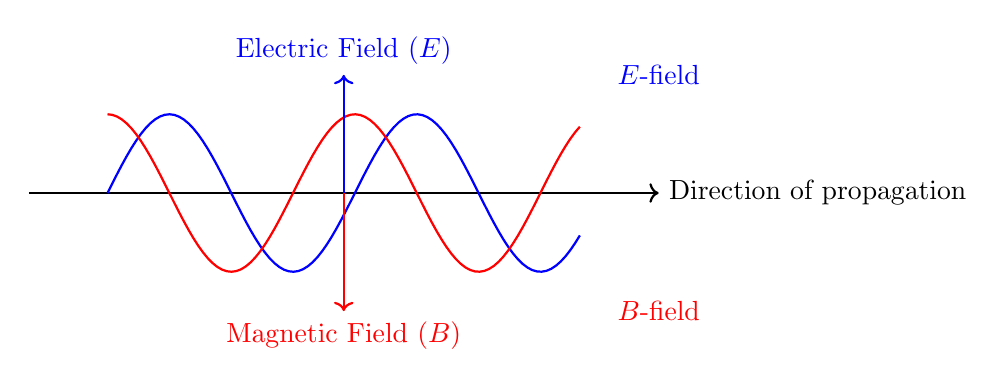
\begin{tikzpicture}[scale=1.0]
		% Wave propagation direction
		\draw[->, thick] (-1, 0) -- (7, 0) node[right] {Direction of propagation};

		% Electric field wave (in blue)
		\draw[blue, thick, domain=0:6, variable=\x, samples=100]
		plot ({\x}, {sin(2 * \x r)});
		\node[blue] at (7, 1.5) {$E$-field};

		% Magnetic field wave (in red)
		\draw[red, thick, domain=0:6, variable=\x, samples=100]
		plot ({\x}, {cos(2 * \x r)});
		\node[red] at (7, -1.5) {$B$-field};

		% Labels
		\draw[->, thick, blue] (3, 0) -- (3, 1.5) node[above] {Electric Field ($E$)};
		\draw[->, thick, red] (3, 0) -- (3, -1.5) node[below] {Magnetic Field ($B$)};
	\end{tikzpicture}
\end{center}

In this diagram, the electric field (\(E\)) oscillates in one plane, while the magnetic field (\(B\)) oscillates in a perpendicular plane. Both fields are sinusoidal and propagate together in the direction shown.

\section{The Wave Equation: \(c = f \lambda\)}

The relationship between the speed of light (\(c\)), the frequency (\(f\)), and the wavelength (\(\lambda\)) of an electromagnetic wave is given by the equation:
\[
	c = f \lambda
\]
where:
\begin{itemize}
	\item \(c\) is the speed of light in a vacuum, approximately \(3 \times 10^8\) m/s,
	\item \(f\) is the frequency of the wave (in Hz),
	\item \(\lambda\) is the wavelength of the wave (in meters).
\end{itemize}

This equation shows that the speed of light is the product of its frequency and wavelength. As the frequency of a wave increases, its wavelength decreases, and vice versa.

\section{The Electromagnetic Spectrum}

The electromagnetic spectrum encompasses all types of electromagnetic radiation, ranging from low-frequency radio waves to high-frequency gamma rays. Below is a diagram showing the range of the spectrum:

\begin{center}
	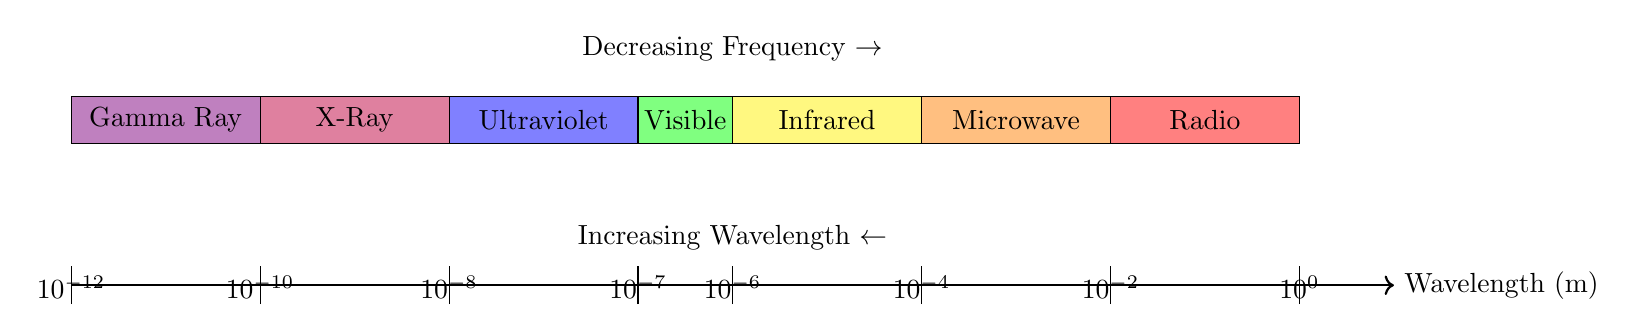
\begin{tikzpicture}[scale=1.2]
		% Spectrum axis

		% Spectrum sections (flipped)
		\draw[fill=violet!50] (0, 0.5) rectangle (2, 1) node[midway] {Gamma Ray};
		\draw[fill=purple!50] (2, 0.5) rectangle (4, 1) node[midway] {X-Ray};
		\draw[fill=blue!50] (4, 0.5) rectangle (6, 1) node[midway] {Ultraviolet};
		\draw[fill=green!50] (6, 0.5) rectangle (7, 1) node[midway] {Visible};
		\draw[fill=yellow!50] (7, 0.5) rectangle (9, 1) node[midway] {Infrared};
		\draw[fill=orange!50] (9, 0.5) rectangle (11, 1) node[midway] {Microwave};
		\draw[fill=red!50] (11, 0.5) rectangle (13, 1) node[midway] {Radio};

		% Labels for increasing frequency and decreasing wavelength
		\node at (7, 1.5) {Decreasing Frequency $\rightarrow$};
		\node at (7, -0.5) {Increasing Wavelength $\leftarrow$};

		% Wavelength ticks
		\draw[thick, ->] (0, -1) -- (14, -1) node[right] {Wavelength (m)};
		\draw (0, -1.2) -- (0, -0.8) node[below] {$10^{-12}$};
		\draw (2, -1.2) -- (2, -0.8) node[below] {$10^{-10}$};
		\draw (4, -1.2) -- (4, -0.8) node[below] {$10^{-8}$};
		\draw (6, -1.2) -- (6, -0.8) node[below] {$10^{-7}$};
		\draw (7, -1.2) -- (7, -0.8) node[below] {$10^{-6}$};
		\draw (9, -1.2) -- (9, -0.8) node[below] {$10^{-4}$};
		\draw (11, -1.2) -- (11, -0.8) node[below] {$10^{-2}$};
		\draw (13, -1.2) -- (13, -0.8) node[below] {$10^{0}$};
	\end{tikzpicture}
\end{center}

The electromagnetic spectrum ranges from long-wavelength, low-frequency waves like radio waves to short-wavelength, high-frequency waves like gamma rays. Visible light is a small portion of the spectrum, spanning from approximately 400 nm (violet) to 700 nm (red) in wavelength.

\section{Absorption Spectrum of Elements}

The absorption spectrum of an element is a unique pattern of dark lines or bands that appear when white light passes through a gas or vapor composed of the element. These dark lines correspond to specific wavelengths of light that have been absorbed by the element's atoms. Understanding absorption spectra is crucial in fields like astronomy and spectroscopy, as they allow scientists to identify elements in stars and distant galaxies.

\subsection{How Absorption Spectra Work}

When white light (which contains all visible wavelengths) passes through a sample of an element in its gaseous state, the electrons in the atoms of that element absorb specific amounts of energy. This energy corresponds to the difference between specific energy levels or orbits of the electrons. 

When electrons absorb this energy, they jump from a lower energy level to a higher energy level, creating an absorption event. Each element has a unique set of energy levels, so the wavelengths absorbed (or "dark lines" in the spectrum) are also unique to each element. These dark lines are referred to as \textbf{absorption lines}.

\subsection{Relationship to Emission Spectrum}

The absorption spectrum is closely related to the \textbf{emission spectrum} of an element. When an electron drops from a higher energy level to a lower one, it emits light at a wavelength corresponding to the energy difference between these levels. In contrast, the absorption spectrum is formed when electrons move from lower to higher energy levels by absorbing light.

The emission lines and absorption lines occur at the same wavelengths for any given element, but they appear differently in the spectra:
\begin{itemize}
    \item \textbf{Emission Spectrum}: Bright lines on a dark background, representing wavelengths emitted by electrons falling to lower energy levels.
    \item \textbf{Absorption Spectrum}: Dark lines on a bright (continuous) background, representing wavelengths absorbed by electrons jumping to higher energy levels.
\end{itemize}

\subsection{Example: Hydrogen Absorption Spectrum}

The hydrogen atom, for example, has a simple absorption spectrum. It consists of a series of dark lines in the visible region, corresponding to the specific wavelengths absorbed by electrons as they move to higher energy levels. The Balmer series is a well-known part of hydrogen's absorption spectrum, with lines appearing in the visible light range.

Below is a simplified representation of the absorption spectrum of hydrogen:
\[
\text{--- --- --- --- ---}
\]
The dark lines represent wavelengths absorbed by the hydrogen atoms.

\subsection{Applications of Absorption Spectra}

Absorption spectra are used in a variety of scientific fields to:
\begin{itemize}
    \item Identify elements present in stars and distant astronomical objects.
    \item Determine the chemical composition of substances.
    \item Study the energy levels and quantum mechanics of atoms and molecules.
\end{itemize}

Since each element has a unique absorption spectrum, this technique allows scientists to detect and analyze the presence of different elements based on the pattern of dark lines that appear in a spectrum.

\begin{center}
    
\begin{tikzpicture}[scale=1.0]
        % Continuous spectrum
        \shade[left color=white, right color=black] (0, 0) rectangle (10, 0.5);
        % Absorption lines
        \draw[very thick, white] (2, 0) -- (2, 0.5);
        \draw[very thick, white] (4, 0) -- (4, 0.5);
        \draw[very thick, white] (6, 0) -- (6, 0.5);
        \draw[very thick, white] (8, 0) -- (8, 0.5);
    \end{tikzpicture}
\end{center}

In this diagram, the gradient from white to black represents the continuous spectrum of light, while the vertical white lines represent absorption lines where specific wavelengths are absorbed by the element.

\end{document}